\documentclass[11pt,a4paper]{article}
\usepackage[T1]{fontenc}
\usepackage[utf8]{inputenc}
\usepackage{lmodern}
\usepackage{textcomp}
\usepackage[left=1.8cm,right=1.8cm,top=2.3cm,bottom=2.2cm,headheight=14pt,headsep=8pt]{geometry}
\usepackage{multicol}
\usepackage{xcolor}
\usepackage{fancyhdr}
\usepackage{graphicx}
\usepackage{array}
\usepackage{amsmath,amssymb}
\usepackage{setspace}
\usepackage{longtable}
\graphicspath{{../}}
\definecolor{ygreen}{RGB}{46,139,87}
\renewcommand{\normalsize}{\fontsize{10.9}{13.4}\selectfont}
\renewcommand{\familydefault}{\rmdefault}
\setlength{\parindent}{0pt}
\setlength{\columnsep}{0.8cm}
\setlength{\columnseprule}{0.4pt}
\setlength{\multicolsep}{3pt plus 1pt minus 1pt}
\renewcommand{\textsubscript}[1]{\ensuremath{_{\text{\fontsize{8}{8}\selectfont #1}}}}
\renewcommand{\textsuperscript}[1]{\ensuremath{^{\text{\fontsize{8}{8}\selectfont #1}}}}
\newcommand{\diqqat}[1]{\par\smallskip\noindent\textbf{Diqqat!} #1\par\medskip}
\newcommand{\javob}{\par\smallskip\noindent\textbf{Javob:} \rule[-2pt]{7.5cm}{0.4pt}\par\smallskip\noindent\textbf{Diqqat!} Javobingizni javoblar varaqasiga ko`chirib yozing.\par\medskip}
\pagestyle{fancy}
\fancyhf{}
\renewcommand{\headrulewidth}{0.4pt}
\fancyhead[L]{\textit{Milliy sertifikat 2026. Kimyo}}
\fancyhead[R]{4-variant}
\fancyfoot[L]{\fontsize{8}{9}\selectfont \textcopyright{} Colba maktabi, 2026}
\fancyfoot[C]{\thepage}
\fancypagestyle{first}{\fancyhf{}\renewcommand{\headrulewidth}{0pt}\fancyfoot[L]{\fontsize{8}{9}\selectfont \textcopyright{} Colba maktabi, 2026}\fancyfoot[C]{\thepage}}
\begin{document}
\normalsize
\thispagestyle{first}
\noindent\fcolorbox{ygreen}{white}{\parbox{\dimexpr\linewidth-2\fboxsep-2\fboxrule\relax}{%
\textbf{\fontsize{13}{15}\selectfont Nazorat testi}\ \textit{\fontsize{10}{12}\selectfont $\cdot$ Aralash test $\cdot$ 4-variant}\hfill
\begin{tabular}[t]{@{}r@{}}\textit{Milliy sertifikat 2026. Kimyo}\\ \textbf{\textit{\fontsize{8}{9}\selectfont Vaqt:}} \textit{\fontsize{10}{12}\selectfont 180 daqiqa}\end{tabular}}}
\par\medskip
\noindent\textit{Davriy jadvaldan foydalanish mumkin.}
\par\medskip
\begin{multicols}{2}
\noindent\textbf{1.} A moddaning parchalanish reaksiyasida konsentratsiyaning vaqt bo`yicha o`zgarishi jadvalda berilgan:
\begin{center}
\renewcommand{\arraystretch}{1.15}
\begin{tabular}{|c|c|}\hline
\textbf{t, min} & \textbf{c, mol/l} \\ \hline
0 & 1,6 \\ \hline
2 & 1,44 \\ \hline
4 & 1,28 \\ \hline
6 & 1,12 \\ \hline
\end{tabular}
\end{center}
2-minutdan 6-minutgacha o`rtacha tezlikni mol/(l$\cdot$min) \textbf{hisoblang.}

\noindent A)~\textsl{0,16} \hfill B)~\textsl{0,08} \hfill C)~\textsl{0,04} \hfill D)~\textsl{0,32}\par
\vspace{4pt}
\noindent\textbf{2.} Qotishmaning massa bo`yicha tarkibi doira diagrammasida ko`rsatilgan.
\begin{center}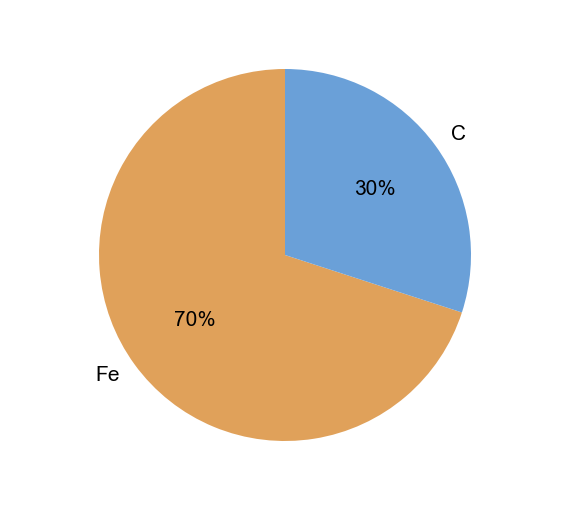
\includegraphics[width=0.86\linewidth]{rasmlar/gen/pi_v04_0.png}\end{center}
Qotishmadagi Fe va C atomlari sonining nisbati (Fe uchun C ga \textbf{bo`lingan)ni toping.}

\noindent A)~\textsl{0,5} \hfill B)~\textsl{2,33} \hfill C)~\textsl{4,67} \hfill D)~\textsl{0,43}\par
\vspace{4pt}
\noindent\textbf{3.} Massa soni 226, zaryadi 88 bo`lgan yadro massa soni 206, zaryadi 82 bo`lgan yadroga aylandi ($\alpha$ va $\beta$\textsuperscript{$-$} parchalanish). Nechta $\alpha$-zarra chiqarilgan?

\noindent A)~\textsl{6} \hfill B)~\textsl{4} \hfill C)~\textsl{7} \hfill D)~\textsl{5}\par
\vspace{4pt}
\noindent\textbf{4.} 30 l CO va 22,5 l O\textsubscript{2} aralashmasi reaksiyaga kirishdi (2CO + O\textsubscript{2} $\to$ 2CO\textsubscript{2}, hamma moddalar bir xil sharoitda gaz holida). Reaksiyadan keyingi gaz aralashmasining \textbf{hajmini (l) aniqlang.}

\noindent A)~\textsl{52,5} \hfill B)~\textsl{30} \hfill C)~\textsl{37,5} \hfill D)~\textsl{7,5}\par
\vspace{4pt}
\noindent\textbf{5.} KMnO\textsubscript{4} tarkibida Mn ning oksidlanish \textbf{darajasini aniqlang.}

\noindent A)~\textsl{$-$2} \hfill B)~\textsl{+7} \hfill C)~\textsl{+4} \hfill D)~\textsl{+3 va +5}\par
\vspace{4pt}
\noindent\textbf{6.} \textit{X}\textasciicircum{}2+ ionida 18 ta elektron va 23 ta neytron bor. \textit{X} atomining nisbiy atom \textbf{massasini aniqlang.}

\noindent A)~\textsl{43} \hfill B)~\textsl{45} \hfill C)~\textsl{41} \hfill D)~\textsl{20}\par
\vspace{4pt}
\noindent\textbf{7.} 2NO + O\textsubscript{2} $\rightleftarrows$ 2NO\textsubscript{2} reaksiyada muvozanat qaror topganda [NO] = 1, [O\textsubscript{2}] = 1, [NO\textsubscript{2}] = 4 mol/l bo`ldi. O\textsubscript{2} ning boshlang`ich \textbf{konsentratsiyasini (mol/l) aniqlang.}

\noindent A)~\textsl{3} \hfill B)~\textsl{1} \hfill C)~\textsl{5} \hfill D)~\textsl{6}\par
\vspace{4pt}
\noindent\textbf{8.} 2SO\textsubscript{2} + O\textsubscript{2} $\rightleftarrows$ 2SO\textsubscript{3} + Q muvozanatni o`ngga siljitadigan \textbf{o`zgarishlarni toping}: 1) katalizator qo`shish; 2) haroratni pasaytirish; 3) bosimni oshirish; 4) bosimni pasaytirish.

\noindent A)~\textsl{1, 2} \hfill B)~\textsl{3, 4} \hfill C)~\textsl{2, 3} \hfill D)~\textsl{1, 3, 4}\par
\vspace{4pt}
\noindent\textbf{9.} CuSO\textsubscript{4}$\cdot$5H\textsubscript{2}O kristallogidratida kristallizatsion suvning massa \textbf{ulushini (\%) aniqlang.}

\noindent A)~\textsl{36} \hfill B)~\textsl{64} \hfill C)~\textsl{18} \hfill D)~\textsl{56,2}\par
\vspace{4pt}
\noindent\textbf{10.} AgNO\textsubscript{3} eritmasi inert elektrodlar yordamida 2 A tok kuchi bilan 965 s elektroliz qilindi. Anodda ajralgan O\textsubscript{2} hajmi (l, n.sh.) \textbf{ni toping.}

\noindent A)~\textsl{0,224} \hfill B)~\textsl{0,056} \hfill C)~\textsl{0,002} \hfill D)~\textsl{0,112}\par
\vspace{4pt}
\noindent\textbf{11.} Zarracha haqida ma'lumot jadvalda berilgan:
\begin{center}
\renewcommand{\arraystretch}{1.15}
\begin{tabular}{|c|c|}\hline
\textbf{Zarracha tarkibi} & \textbf{Soni} \\ \hline
proton & 30 \\ \hline
neytron & 34 \\ \hline
elektron & 29 \\ \hline
\end{tabular}
\end{center}
Shu zarrachaning massa \textbf{sonini aniqlang.}

\noindent A)~\textsl{64} \hfill B)~\textsl{65} \hfill C)~\textsl{59} \hfill D)~\textsl{60}\par
\vspace{4pt}
\noindent\textbf{12.} Qaysi juftliklarda reaksiya boradi? 1) Mg va FeSO\textsubscript{4}; 2) Cu va AgNO\textsubscript{3}; 3) Zn va CuSO\textsubscript{4}; 4) Cu va ZnSO\textsubscript{4}

\noindent A)~\textsl{2, 3} \hfill B)~\textsl{1, 2, 3} \hfill C)~\textsl{1, 2} \hfill D)~\textsl{2, 4}\par
\vspace{4pt}
\noindent\textbf{13.} Rasmda indikatorlarning pH ga bog`liq rangi ko`rsatilgan.
\begin{center}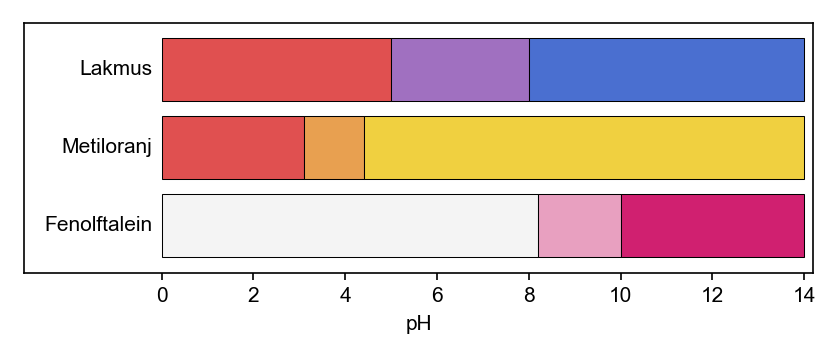
\includegraphics[width=0.86\linewidth]{rasmlar/gen/in_352151.png}\end{center}
pH = 2 bo`lgan eritmada lakmus qanday rangga kiradi?

\noindent\begin{tabular}{@{}p{0.47\linewidth}@{}p{0.47\linewidth}@{}}
A)~\textsl{zarg`aldoq} & B)~\textsl{binafsha} \\
C)~\textsl{qizil} & D)~\textsl{och pushti} \\
\end{tabular}\par
\vspace{4pt}
\noindent\textbf{14.} Qaysi juftliklar o`zaro reaksiyaga kirishadi? 1) CuSO\textsubscript{4} va NaOH; 2) Zn va NaOH; 3) MgCl\textsubscript{2} va KNO\textsubscript{3}; 4) Cu va HNO\textsubscript{3}(kons.)

\noindent A)~\textsl{1, 4} \hfill B)~\textsl{1, 3} \hfill C)~\textsl{2, 3, 4} \hfill D)~\textsl{1, 2, 4}\par
\vspace{4pt}
\noindent\textbf{15.} 2KClO\textsubscript{3} $\to$ 2KCl + 3O\textsubscript{2} reaksiyasida 245 g KClO\textsubscript{3} ishtirok etdi. O\textsubscript{2} \textbf{hajmini (l, n.sh.) toping.}

\noindent A)~\textsl{29,87} \hfill B)~\textsl{67,2} \hfill C)~\textsl{134,4} \hfill D)~\textsl{33,6}\par
\vspace{4pt}
\noindent\textbf{16.} K\textsubscript{2}SO\textsubscript{4} tarkibidagi kaliy ning massa \textbf{ulushini (\%) aniqlang.}

\noindent A)~\textsl{44,8} \hfill B)~\textsl{22,4} \hfill C)~\textsl{89,7} \hfill D)~\textsl{2,2}\par
\vspace{4pt}
\noindent\textbf{17.} AgNO\textsubscript{3} qizdirilganda qanday moddalar hosil bo`ladi?

\noindent\begin{tabular}{@{}p{0.47\linewidth}@{}p{0.47\linewidth}@{}}
A)~\textsl{CuO, NO\textsubscript{2} va O\textsubscript{2}} & B)~\textsl{KNO\textsubscript{2} va O\textsubscript{2}} \\
C)~\textsl{Ag, NO\textsubscript{2} va O\textsubscript{2}} & D)~\textsl{ZnO, NO\textsubscript{2} va O\textsubscript{2}} \\
\end{tabular}\par
\vspace{4pt}
\noindent\textbf{18.} Reaksiya tenglamasi: FeS + 2HCl $\to$ FeCl\textsubscript{2} + H\textsubscript{2}S. Reaksiyaga 11,2 l (n.sh.) HCl kirishdi. FeCl\textsubscript{2} \textbf{massasini (g) hisoblang.}

\noindent A)~\textsl{127} \hfill B)~\textsl{63,5} \hfill C)~\textsl{31,75} \hfill D)~\textsl{15,88}\par
\vspace{4pt}
\noindent\textbf{19.} Reaksiya tenglamasi: NH\textsubscript{4}Cl + NaOH $\to$ NaCl + NH\textsubscript{3} + H\textsubscript{2}O. Reaksiyaga tarkibida 60\% aralashma bo`lgan 40 g namuna (asosiy modda NaOH) kirishdi. NH\textsubscript{3} \textbf{hajmini (l, n.sh.) hisoblang.}

\noindent A)~\textsl{17,92} \hfill B)~\textsl{8,96} \hfill C)~\textsl{4,48} \hfill D)~\textsl{13,44}\par
\vspace{4pt}
\noindent\textbf{20.} C\textsubscript{3}H\textsubscript{7}OH tarkibli spirtlarning izomerlari soni nechta?

\noindent A)~\textsl{3} \hfill B)~\textsl{1} \hfill C)~\textsl{4} \hfill D)~\textsl{2}\par
\vspace{4pt}
\noindent\textbf{21.} Alken, alkadiyen va alkinlar haqida qaysi fikrlar to`g`ri? 1) Kauchuk izoprenning polimeri; 2) Alkenlarda $\pi$-bog` yo`q; 3) Alkinlar uchun umumiy formula CnH\textsubscript{2}n+2; 4) Propenga HBr birikishi Markovnikov qoidasiga bo`ysunadi

\noindent A)~\textsl{1, 4} \hfill B)~\textsl{2, 3, 4} \hfill C)~\textsl{1, 2, 3} \hfill D)~\textsl{1, 3}\par
\vspace{4pt}
\noindent\textbf{22.} C\textsubscript{2}H\textsubscript{2} + H\textsubscript{2}O $\to$ CH\textsubscript{3}CHO reaksiyasida 52 g C\textsubscript{2}H\textsubscript{2} ishtirok etdi. CH\textsubscript{3}CHO \textbf{massasini (g) toping.}

\noindent A)~\textsl{176} \hfill B)~\textsl{44} \hfill C)~\textsl{132} \hfill D)~\textsl{88}\par
\vspace{4pt}
\noindent\textbf{23.} Spirt va fenollar haqida qaysi fikrlar to`g`ri? 1) Fenol FeCl\textsubscript{3} bilan binafsha rang beradi; 2) Uchlamchi spirtlar oson oksidlanadi; 3) Fenol Cu(OH)\textsubscript{2} ni eritib ko`k kompleks hosil qiladi; 4) Glitserin Cu(OH)\textsubscript{2} bilan ko`k kompleks hosil qiladi

\noindent A)~\textsl{1, 4} \hfill B)~\textsl{1, 2, 3} \hfill C)~\textsl{1, 3, 4} \hfill D)~\textsl{1, 3}\par
\vspace{4pt}
\noindent\textbf{24.} 18 g glyukoza Ag\textsubscript{2}O ning ammiakli eritmasi bilan to`liq oksidlanganda hosil bo`lgan kumush \textbf{massasini (g) aniqlang.}

\noindent A)~\textsl{10,8} \hfill B)~\textsl{43,2} \hfill C)~\textsl{21,6} \hfill D)~\textsl{18}\par
\vspace{4pt}
\noindent\textbf{25.} Karbon kislotalar haqida qaysi fikrlar to`g`ri? 1) Chumoli kislota "kumush ko`zgu" reaksiyasini beradi; 2) Sirka angidrid ikki molekula sirka kislotadan suv chiqib hosil bo`ladi; 3) Benzoy kislota Na\textsubscript{2}CO\textsubscript{3} bilan reaksiyaga kirishmaydi; 4) Qattiq suvda sovun yaxshi ko`piklanadi

\noindent A)~\textsl{3, 4} \hfill B)~\textsl{2, 3} \hfill C)~\textsl{1, 2, 3} \hfill D)~\textsl{1, 2}\par
\vspace{4pt}
\noindent\textbf{26.} CH\textsubscript{3}COOCH\textsubscript{3} + NaOH $\to$ CH\textsubscript{3}COONa + CH\textsubscript{3}OH jarayoni uchun 20 g NaOH olingan (unum 90\%). CH\textsubscript{3}COONa \textbf{massasini (g) aniqlang.}

\noindent A)~\textsl{41} \hfill B)~\textsl{36,9} \hfill C)~\textsl{73,8} \hfill D)~\textsl{18,45}\par
\vspace{4pt}
\noindent\textbf{27.} Quyidagi birikmalardan qaysi biri karbon kislota sinfiga kiradi?

\noindent A)~\textsl{C\textsubscript{2}H\textsubscript{5}OH} \hfill B)~\textsl{C\textsubscript{12}H\textsubscript{22}O\textsubscript{11}} \hfill C)~\textsl{CH\textsubscript{3}COOH} \hfill D)~\textsl{C\textsubscript{6}H\textsubscript{12}O\textsubscript{6}}\par
\vspace{4pt}
\noindent\textbf{28.} 11,7 g valin HCl bilan reaksiyaga kirishganda hosil bo`lgan tuz \textbf{massasini (g) aniqlang.}

\noindent A)~\textsl{11,7} \hfill B)~\textsl{3,65} \hfill C)~\textsl{30,7} \hfill D)~\textsl{15,35}\par
\vspace{4pt}
\noindent\textbf{29.} C\textsubscript{2}H\textsubscript{2} + HCl $\to$ C\textsubscript{2}H\textsubscript{3}Cl reaksiyasida 44,8 l (n.sh.) HCl ishtirok etdi. C\textsubscript{2}H\textsubscript{2} \textbf{hajmini (l, n.sh.) toping.}

\noindent A)~\textsl{89,6} \hfill B)~\textsl{22,4} \hfill C)~\textsl{67,2} \hfill D)~\textsl{44,8}\par
\vspace{4pt}
\noindent\textbf{30.} Cu\textsuperscript{2+} ionini aniqlash uchun qaysi reagent mos va qanday belgi kuzatiladi?
\noindent A)~\textsl{NaOH: oq-yashil cho`kma (Fe(OH)\textsubscript{2})}\par
\noindent B)~\textsl{NaOH: havorang cho`kma (Cu(OH)\textsubscript{2})}\par
\noindent C)~\textsl{HCl: oq cho`kma (AgCl)}\par
\noindent D)~\textsl{AgNO\textsubscript{3}: och sariq cho`kma (AgBr)}\par
\vspace{4pt}
\noindent\textbf{31.} 250 g 10\% li CuSO\textsubscript{4} eritmasidan 50 g suv bug`latildi. Qolgan eritmadagi tuzning massa \textbf{ulushini (\%) toping.}

\noindent A)~\textsl{8,33} \hfill B)~\textsl{12,5} \hfill C)~\textsl{2} \hfill D)~\textsl{10}\par
\vspace{4pt}
\noindent\textbf{32.} Rasmdagi asbobda 6,5 g rux xlorid kislota bilan reaksiyaga kirishdi (Zn + 2HCl $\to$ ZnCl\textsubscript{2} + H\textsubscript{2}). Ajralgan vodorodning \textbf{hajmini (l, n.sh.) aniqlang.}
\begin{center}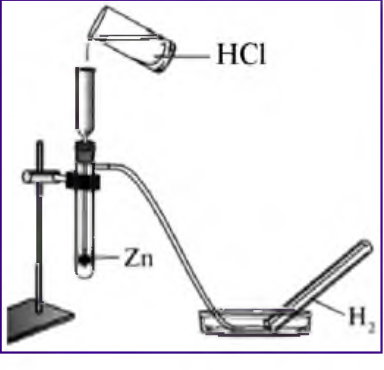
\includegraphics[width=0.86\linewidth]{rasmlar/darslik/d_vodorod.png}\end{center}

\noindent A)~\textsl{4,48} \hfill B)~\textsl{1,12} \hfill C)~\textsl{2,24} \hfill D)~\textsl{0,1   ---}\par
\vspace{4pt}
\end{multicols}
\medskip
\noindent\setlength{\fboxsep}{0pt}\fbox{\begin{tabular}{p{0.74\linewidth}|p{0.2\linewidth}}
\parbox[t]{0.72\linewidth}{\vspace{3pt}\textbf{Topshiriqlar (33--35) va javob variant (A--F)larini o`zaro to`g`ri moslashtiring.} NaBr va KCl dan iborat 12,6 g aralashma suvda eritilib, mo`l AgNO\textsubscript{3} eritmasi qo`shildi; hosil bo`lgan cho`kmalarning umumiy massasi 23,75 g.
\vspace{3pt}} & \parbox[t]{0.19\linewidth}{\vspace{3pt}A~\textsl{5,15}\\[3pt]
B~\textsl{7,73}\\[3pt]
C~\textsl{14,35}\\[3pt]
D~\textsl{11,48}\\[3pt]
E~\textsl{255}\\[3pt]
F~\textsl{127,5}}\\ \hline
\parbox[t]{0.72\linewidth}{\vspace{2pt}\textbf{33. Aralashmadagi NaBr massasini (g) aniqlang.}\vspace{2pt}} & \\ \hline
\parbox[t]{0.72\linewidth}{\vspace{2pt}\textbf{34. Sarflangan 10\% li AgNO\textsubscript{3} eritmasining massasini (g) aniqlang (M(AgNO\textsubscript{3}) = 170 g/mol).}\vspace{2pt}} & \\ \hline
\parbox[t]{0.72\linewidth}{\vspace{2pt}\textbf{35. Eritmada hosil bo`lgan nitratlarning umumiy massasini (g) aniqlang.}\vspace{2pt}} & 
\end{tabular}}
\par\bigskip
\noindent\textbf{36.} H\textsubscript{2}S + HNO\textsubscript{3} $\to$ H\textsubscript{2}SO\textsubscript{4} + NO\textsubscript{2} + H\textsubscript{2}O reaksiya tenglamasini tenglang. Reagentlar (chap qism) koeffitsiyentlari \textbf{yig`indisini toping.}
\javob
\noindent\textbf{37.} 1 l hajmli yopiq idishda 4 mol N\textsubscript{2}O\textsubscript{4} qizdirilganda N\textsubscript{2}O\textsubscript{4} $\rightleftarrows$ 2NO\textsubscript{2} muvozanati qaror topdi. Muvozanat aralashmasining vodorodga nisbatan zichligi 36,8 ga teng. Shu haroratdagi muvozanat \textbf{konstantasini (K, mol/l) hisoblang.}
\javob
\noindent\textbf{38.} Alyuminiy va kalsiy dan iborat 6,7 g aralashma mo`l xlorid kislotada eritilganda 5,6 l (n.sh.) vodorod ajraldi. Aralashmadagi alyuminiyning massa \textbf{ulushini (\%) aniqlang.}
\javob
\noindent\textbf{39.} Etilen va asetilendan iborat 4,48 l (n.sh.) aralashma bromli suvdan o`tkazilganda 40 g brom yutildi. Aralashmadagi asetilenning \textbf{hajmini (l, n.sh.) toping.}
\javob
\noindent\textbf{40.} 17,8 g tristearin mo`l NaOH eritmasi bilan to`liq gidrolizlandi (sovun unumi 90\%). Hosil bo`lgan natriy stearat (M = 306 g/mol) \textbf{massasini (g) toping.}
\javob
\par\bigskip\begin{center}\textbf{\fontsize{13}{15}\selectfont YOZMA ISH}\end{center}
\noindent\textbf{41.} \textbf{Topshiriqni bajarish jarayonida barcha reaksiya tenglamalarini yozing. Miqdoriy va arifmetik hisoblashlarni (unga asos bo`lgan usul yoki formulani ko`rsatgan holda) uzviy ketma-ketlikda bajaring.}\par\smallskip
14,3 g Na\textsubscript{2}CO\textsubscript{3}$\cdot$10H\textsubscript{2}O 400 g suvda eritildi.\par
\noindent 1)Hosil bo`lgan eritmadagi Na\textsubscript{2}CO\textsubscript{3} ning massa ulushini (\%) toping.\par
\noindent 2)Eritmaga mo`l CaCl\textsubscript{2} qo`shildi. Hosil bo`lgan cho`kma massasini (g) toping. Eritmadagi kation miqdorini (mol) ham toping.\par
\noindent 3)Xuddi shunday eritmaga mo`l HCl qo`shilganda ajralgan gazning hajmini (l, n.sh.) hisoblang.\par
\noindent 4)Eritmani to`liq neytrallash (Na\textsubscript{2}CO\textsubscript{3} + 2HCl $\to$ 2NaCl + CO\textsubscript{2} + H\textsubscript{2}O) uchun 10\% li HCl eritmasidan necha gramm kerak? Dastlabki eritma massasini (g) ham ayting.\par
\noindent 5)Kristallogidratdagi kristallizatsion suvning massa ulushini (\%) va unda suv molekulalari sonini toping. Shu miqdor kristallogidrat suvsizlantirilganda massa necha gramm kamayadi?\par
\diqqat{Mazkur topshiriq kengaytirilgan javobni talab etib, uning yechilish usuli va shu usul asosidagi barcha hisoblash amallari javoblar varaqasida aks etishi lozim.}
\noindent\textbf{42.} Quyidagi o`zgarishlar zanjirida \textit{X}, \textit{Y}, \textit{Z} noma'lum organik moddalar:\par
\[\setlength{\fboxsep}{0pt}\text{C\textsubscript{6}H\textsubscript{12}O\textsubscript{6}}\xrightarrow{\text{bijg`ish}}\text{\textit{X}}\xrightarrow{\text{H\textsubscript{2}SO\textsubscript{4} (kons.), 170 \textdegree{}C}}\text{\textit{Y}}\xrightarrow{\text{Br\textsubscript{2}}}\text{C\textsubscript{2}H\textsubscript{4}Br\textsubscript{2}}\]
\noindent 1)C\textsubscript{6}H\textsubscript{12}O\textsubscript{6} $\to$ \textit{X} : reaksiya tenglamasini yozing; hosil bo`lgan moddani nomlang.\par
\noindent 2)\textit{X} $\to$ \textit{Y} : reaksiya tenglamasini yozing; hosil bo`lgan moddani nomlang.\par
\noindent 3)\textit{Y} $\to$ C\textsubscript{2}H\textsubscript{4}Br\textsubscript{2} : reaksiya tenglamasini yozing; hosil bo`lgan moddani nomlang.\par
\diqqat{Mazkur topshiriq kengaytirilgan javobni talab etib, uning yechilish usuli va shu usul asosidagi barcha hisoblash amallari javoblar varaqasida aks etishi lozim.}
\noindent\textbf{43.} \textbf{Topshiriqni bajarish jarayonida barcha reaksiya tenglamalarini yozing. Miqdoriy va arifmetik hisoblashlarni (unga asos bo`lgan usul yoki formulani ko`rsatgan holda) uzviy ketma-ketlikda bajaring.}\par\smallskip
5,6 g temir mo`l xlorda yondirildi. Hosil bo`lgan tuz suvda eritilib, avval ishqor bilan, so`ng boshqa porsiyasi KI eritmasi bilan ta'sirlashtirildi.\par
\noindent 1)Reaksiya tenglamasini yozing. Sarflangan xlor hajmini (l, n.sh.) va hosil bo`lgan tuz massasini (g) toping. Hosil bo`lgan FeCl\textsubscript{3} miqdorini (mol) ham toping.\par
\noindent 2)Tuz eritmasiga mo`l NaOH qo`shilganda hosil bo`lgan cho`kma massasini (g) aniqlang.\par
\noindent 3)Cho`kma qizdirilganda hosil bo`ladigan oksid massasini (g) hisoblang.\par
\noindent 4)Tuzning shunday miqdoriga mo`l KI qo`shilganda ajraladigan yod massasini (g) toping (2FeCl\textsubscript{3} + 2KI $\to$ 2FeCl\textsubscript{2} + 2KCl + I\textsubscript{2}).\par
\noindent 5)Hosil bo`lgan FeCl\textsubscript{3} eritmasiga temir qo`shilib FeCl\textsubscript{2} hosil qilindi (2FeCl\textsubscript{3} + Fe $\to$ 3FeCl\textsubscript{2}). Sarflangan temir massasini (g) toping.\par
\diqqat{Mazkur topshiriq kengaytirilgan javobni talab etib, uning yechilish usuli va shu usul asosidagi barcha hisoblash amallari javoblar varaqasida aks etishi lozim.}
\newpage
\noindent\textbf{\fontsize{13}{15}\selectfont Nazorat testi}\ \textit{$\cdot$ 4-variant}\hfill \textbf{Javoblar kaliti}\par\smallskip\hrule\smallskip
\textit{Faqat o`qituvchi uchun.}\par\medskip
\noindent\textbf{1--32-savollar}\par\smallskip
\noindent\begin{tabular}{|c|c|c|c|c|c|c|c|c|c|c|c|c|c|c|c|}\hline
\textbf{1} & \textbf{2} & \textbf{3} & \textbf{4} & \textbf{5} & \textbf{6} & \textbf{7} & \textbf{8} & \textbf{9} & \textbf{10} & \textbf{11} & \textbf{12} & \textbf{13} & \textbf{14} & \textbf{15} & \textbf{16}\\\hline
\textsl{B} & \textsl{A} & \textsl{D} & \textsl{C} & \textsl{B} & \textsl{A} & \textsl{A} & \textsl{C} & \textsl{A} & \textsl{D} & \textsl{A} & \textsl{B} & \textsl{C} & \textsl{D} & \textsl{B} & \textsl{A}\\\hline
\textbf{17} & \textbf{18} & \textbf{19} & \textbf{20} & \textbf{21} & \textbf{22} & \textbf{23} & \textbf{24} & \textbf{25} & \textbf{26} & \textbf{27} & \textbf{28} & \textbf{29} & \textbf{30} & \textbf{31} & \textbf{32}\\\hline
\textsl{C} & \textsl{C} & \textsl{B} & \textsl{D} & \textsl{A} & \textsl{D} & \textsl{A} & \textsl{C} & \textsl{D} & \textsl{B} & \textsl{C} & \textsl{D} & \textsl{D} & \textsl{B} & \textsl{B} & \textsl{C}\\\hline
\end{tabular}\par\medskip
\noindent\textbf{33--35-savollar}\par\smallskip
\noindent\begin{tabular}{|c|c|c|}\hline \textbf{No} & \textbf{Javob} & \textbf{Qiymat}\\\hline
33 & \textsl{A} & 5,15\\\hline
34 & \textsl{E} & 255\\\hline
35 & \textsl{C} & 14,35\\\hline
\end{tabular}\par\medskip
\noindent\textbf{36--40-savollar}\par\smallskip
\noindent\begin{tabular}{|c|c|}\hline \textbf{No} & \textbf{To`g`ri javob}\\\hline
36 & 9\\\hline
37 & 1,333\\\hline
38 & 40,3\\\hline
39 & 1,12\\\hline
40 & 16,52\\\hline
\end{tabular}\par\medskip
\noindent\textbf{41--43-topshiriqlar: qisqa yechim}\par\smallskip
\noindent\textbf{41-topshiriq.}\par
\noindent 1) m(Na\textsubscript{2}CO\textsubscript{3}) = 0,05$\cdot$106 = 5,3 g; m(eritma) = 14,3 + 400 = 414,3 g; $\omega$ = \textbf{1,28\%}\par
\noindent 2) Na\textsubscript{2}CO\textsubscript{3} + CaCl\textsubscript{2} $\to$ CaCO\textsubscript{3}$\downarrow$ + 2NaCl: 0,05 mol $\cdot$ 100 = \textbf{5 g}; n(kation) = \textbf{0,05 mol}\par
\noindent 3) Na\textsubscript{2}CO\textsubscript{3} + 2HCl $\to$ 2NaCl + CO\textsubscript{2}$\uparrow$ + H\textsubscript{2}O: \textbf{1,12 l}\par
\noindent 4) n(HCl) = 0,1 mol = 3,65 g; 3,65/0,1 = \textbf{36,5 g}; m(eritma) = 14,3 + 400 = \textbf{414,3 g}\par
\noindent 5) $\omega$(H\textsubscript{2}O) = (286 $-$ 106)/286 = \textbf{62,9\%}; suv molekulalari: \textbf{10} ta; $\Delta$m = 0,05$\cdot$(286 $-$ 106) = \textbf{9 g}\par
\noindent Jami: M 15 + A 10 = 25 ball.\par
\noindent\textbf{42-topshiriq.}\par
\noindent 1) C\textsubscript{6}H\textsubscript{12}O\textsubscript{6} + bijg`ish $\to$ C\textsubscript{2}H\textsubscript{5}OH (etanol)\par
\noindent 2) C\textsubscript{2}H\textsubscript{5}OH + H\textsubscript{2}SO\textsubscript{4} (kons.), 170 \textdegree{}C $\to$ C\textsubscript{2}H\textsubscript{4} (etilen)\par
\noindent 3) C\textsubscript{2}H\textsubscript{4} + Br\textsubscript{2} $\to$ C\textsubscript{2}H\textsubscript{4}Br\textsubscript{2} (1,2-dibrometan)\par
\noindent Jami 25 ball.\par
\noindent\textbf{43-topshiriq.}\par
\noindent 1) 2Fe + 3Cl\textsubscript{2} $\to$ 2FeCl\textsubscript{3}: \textit{V}(Cl\textsubscript{2}) = 0,1$\cdot$1,5$\cdot$22,4 = \textbf{3,36 l}; m(FeCl\textsubscript{3}) = \textbf{16,25 g}; n(FeCl\textsubscript{3}) = n(Fe) = \textbf{0,1 mol}\par
\noindent 2) FeCl\textsubscript{3} + 3NaOH $\to$ Fe(OH)\textsubscript{3}$\downarrow$ + 3NaCl: 0,1$\cdot$107 = \textbf{10,7 g}\par
\noindent 3) 2Fe(OH)\textsubscript{3} $\to$ Fe\textsubscript{2}O\textsubscript{3} + 3H\textsubscript{2}O: n = 0,05 mol $\to$ \textbf{8 g}\par
\noindent 4) n(I\textsubscript{2}) = 0,1/2 = 0,05 mol $\to$ \textbf{12,7 g}\par
\noindent 5) n(Fe) = 0,1/2 = 0,05 mol $\to$ \textbf{2,8 g}\par
\noindent Jami: M 15 + A 10 = 25 ball.\par
\par\bigskip\noindent\textbf{Mavzular taqsimoti}\par\smallskip
{\small\noindent\begin{longtable}{|c|p{7.2cm}|p{5.4cm}|c|}\hline \textbf{No} & \textbf{Mavzu} & \textbf{Tekshiriladigan ko`nikma} & \textbf{Ball}\\\hline
1 & Tirkashev VI bob (tezlik, jadval) & Jadval tahlili & 1\\\hline
2 & 8-sinf (mol, diagramma) & Grafik tahlili & 1\\\hline
3 & 11-sinf 1-bob (yadro reaksiyalari) & Bilim va tushunish & 1\\\hline
4 & 8-sinf (Gey-Lyussak, Avogadro) & Hisoblash va masala yechish & 1\\\hline
5 & 8-sinf; Tirkashev \textit{V} bob (oksidlanish darajasi) & Bilim va tushunish & 1\\\hline
6 & 8-sinf (atom tuzilishi) & Hisoblash va masala yechish & 1\\\hline
7 & Tirkashev VI bob & Hisoblash va masala yechish & 1\\\hline
8 & Tirkashev VI bob (Le-Shatelye) & Bilim va tushunish & 1\\\hline
9 & 7-sinf; Tirkashev (kristallogidrat) & Hisoblash va masala yechish & 1\\\hline
10 & 11-sinf 8-bob (Faradey qonunlari); Tirkashev \textit{V} bob & Hisoblash va masala yechish & 1\\\hline
11 & 8-sinf (atom tuzilishi, jadval) & Jadval tahlili & 1\\\hline
12 & Tashev; 9-sinf (kuchlanish qatori) & Bilim va tushunish & 1\\\hline
13 & 8-sinf (indikatorlar) & Rasm bo`yicha tahlil & 1\\\hline
14 & 9-sinf; Tashev (anorganik birikmalar xossalari) & Bilim va tushunish & 1\\\hline
15 & 9-sinf; Tirkashev (genetik zanjir/reaksiya turlari, hisob) & Hisoblash va masala yechish & 1\\\hline
16 & Tashev (o`g`itlar) & Hisoblash va masala yechish & 1\\\hline
17 & Tashev (nitratlar) & Bilim va tushunish & 1\\\hline
18 & 9-sinf; Tirkashev (S/SO\textsubscript{2}/H\textsubscript{2}SO\textsubscript{4}, hisob) & Hisoblash va masala yechish & 1\\\hline
19 & 9-sinf; Tirkashev (N/NH\textsubscript{3}/HNO\textsubscript{3}, hisob) & Hisoblash va masala yechish & 1\\\hline
20 & 10-sinf \S{}6, \S{}12, \S{}20, \S{}28 (izomeriya) & Bilim va tushunish & 1\\\hline
21 & 10-sinf (mavzuga oid paragraflar); Abdusamatov & Bilim va tushunish & 1\\\hline
22 & 10-sinf (aren, hisob) & Hisoblash va masala yechish & 1\\\hline
23 & 10-sinf (mavzuga oid paragraflar); Abdusamatov & Bilim va tushunish & 1\\\hline
24 & 10-sinf \S{}24; \S{}26; \S{}30 (kumush ko`zgu) & Hisoblash va masala yechish & 1\\\hline
25 & 10-sinf (mavzuga oid paragraflar); Abdusamatov & Bilim va tushunish & 1\\\hline
26 & 10-sinf (efir, hisob) & Hisoblash va masala yechish & 1\\\hline
27 & 10-sinf (organik birikmalar sinflari) & Bilim va tushunish & 1\\\hline
28 & 10-sinf \S{}34 & Hisoblash va masala yechish & 1\\\hline
29 & 10-sinf (pol, hisob) & Hisoblash va masala yechish & 1\\\hline
30 & 9-sinf (sifat reaksiyalar) & Bilim va tushunish & 1\\\hline
31 & Tirkashev III bob (eritmalar) & Hisoblash va masala yechish & 1\\\hline
32 & 7-sinf (28-rasm); 8-sinf (stexiometriya) & Rasm bo`yicha tahlil & 1\\\hline
33--35 & Aralash masala (moslashtirish) & Ko`p bosqichli hisob & 3\\\hline
36--40 & Qisqa javobli masalalar & Hisoblash & 5\\\hline
41--43 & Yozma ish & Usul va hisob (M, A) & 75\\\hline
\end{longtable}}
\end{document}
